\documentclass{article}[10pt]
\setlength{\evensidemargin}{0in}
\setlength{\oddsidemargin}{0in}
\setlength{\textwidth}{6.5in}
\setlength{\textheight}{9in}
\setlength{\topmargin}{-.75in}
\usepackage{graphicx}
\usepackage{amsmath}
\usepackage{amsthm}
\usepackage{amssymb}
\usepackage{tikz}
\usetikzlibrary{calc}
\usetikzlibrary{arrows, decorations.markings}
\usetikzlibrary{arrows.meta}
\usepackage{enumerate}
\usepackage{datetime}
\usepackage{natbib}
\usepackage{array}
\usepackage{hyperref}
\usepackage{color}
\hypersetup{
colorlinks= true,
allcolors = blue
}
\usepackage{arev} % excellent sans-serif font that has its own math mode font!
\newtheorem{theorem}{Theorem}
\usepackage{floatrow}

\title{171.107 Midterm 1 Solutions}
\date{September 30, 2016}
%\author{Michael Busch, Alexander de la Vega and Hsiang-Chih Hwang}

\begin{document}
\maketitle

\tikzset{->-/.style={decoration={
  markings,
  mark=at position #1 with {\arrow{>}}},postaction={decorate}}}
  
\begin{enumerate}

% question 1
\item  Two cars with identical mass travel around concentric circular tracks, as shown in the picture below. The coefficients of friction between the
cars' tires and the tracks are identical in the two cases. (Note that the centripetal force is provided by friction. 

% tikzpicture
\begin{center}
\begin{tikzpicture}

\draw [fill=gray] (0,0) circle (2.5);
\draw [fill=white] (0,0) circle (2); 

\draw [fill=gray] (0,0) circle (1.5);
\draw [fill=white] (0,0) circle (1); 

\draw [color=yellow, dashed, thick=2] circle (2.25);
\draw [color=yellow, dashed, thick=2] circle (1.25);

\node [rotate=90] at (2.25, 0) {\includegraphics[width=0.3in]{red_car.png}};
\node [rotate=90] at (1.25, 0) {\includegraphics[width=0.3in]{red_car.png}};

\end{tikzpicture}
\end{center}

\begin{enumerate}[(a)]

% 1 a
\item {[}7.5 pts] \label{question:1:a} Which car can travel at a larger speed without skidding off its track?

\begin{enumerate}[i]

\item The car on the inner track.

\item The car in the outer track.

\item The cars have the same maximum speed above which they skid.

\end{enumerate}

Explain your answer. \\

% solution 1 a
{\color{red}The car on the outer track (\framebox[1.1\width]{choice ii}) can travel at a higher speed without skidding. At the maximum speed before skidding, the 
force arising from centripetal acceleration is equal to that of the force of friction, that is,

$$ \frac{mv^2}{r} = mg \mu_s,$$

so

$$ \frac{v^2}{r} = g \mu_s \Longrightarrow v = \sqrt{g\mu_s r}.$$

As $v \propto \sqrt{r}$, the car on the outer track can travel a larger speed without skidding.} \\

% 1 b
\item {[}7.5 pts] Which car can travel at a larger angular speed without skidding off of its track?

\begin{enumerate}[i]

\item The car on the inner track.

\item The car in the outer track.

\item The cars have the same maximum angular speed above which they skid.

\end{enumerate}

Explain your answer. \\

% solution 1 b
{\color{red} The car on the inner track (\framebox[1.1\width]{choice i}) can travel a larger angular speed without skidding. From Question \ref{question:1:a}, we found
$v = \sqrt{g \mu_s r}$, and as $\omega = \frac{v}{r}$, we have that

$$ \omega = \frac{\sqrt{g \ mu_s r}}{r} \Longrightarrow \omega \propto \frac{1}{\sqrt{r}}.$$

As such, the car on the smaller track can travel a larger angular speed without skidding.} \\

\end{enumerate} % end 1

% question 2
\item A gun is located on the side of a steep 45$^\circ$ hill. For simplicity, assume that the gun is at the origin of a coordinate system as shown below
and ignore the length of the gun barrel.

\begin{center}
\begin{tikzpicture}

% axes
\draw [-triangle 45=0.25] (0,0) -- (0,3); % y
\draw [-triangle 45 =0.25] (0,0) -- (3,0); % x
\node at (3.1, 0) {x};
\node at (-.2, 2.6) {y};

% hillside
\draw [color=blue, thick=2] (-2, 2) -- (3, -3); 
\node [rotate=-45, color=blue] at (-1.2, 1.5) {hillside};
\draw (3, -3) -- (1, -3);
\draw [-triangle 45=0.25] (3, -3) ++(135:1) arc(135:180:1);
\draw [-triangle 45=0.25] (3, -3) ++(180:1) arc(180:135:1);
\node at (1.7, -2.5) {$45^\circ$};

% other lines
\draw [color=green, thick=2, dashed, domain=0:0.392, -triangle 45=0.2] plot (\x, {25.5 * \x - 65 * \x ^ 2});
\node [color=green] at (.6, 1.5) {h};
\draw [color=orange, dashed, thick=2, domain=0:2.6, -triangle 45=0.2] plot (\x, {1.65 * \x - 1 * \x ^ 2});
\draw [color=orange, -triangle 45=0.25] (.1, 2.6) -- (2.6, 2.6);
\draw [color=orange, -triangle 45=0.25] (2.6, 2.6) -- (.1, 2.6);
\draw [dotted, thick=2] (2.7, 3) -- (2.7, -2.7);
\node [color=orange] at (1.3, 2.9) {R};

% gun
\draw [color=orange, thick=2] (.1, -.1) -- (-.1, -.1) -- (-.1, 1) -- (.1, 1) -- (.1, -.1);
\draw [color=orange, thick=2, rotate=-45] (.1, -.1) -- (-.1, -.1) -- (-.1, 1) -- (.1, 1) -- (.1, -.1);
\node [color=orange] at (-.4, -.4) {gun};
\draw [-triangle 45=0.25] (0,0) ++(0:1.1) arc(0:45:1.1);
\draw [-triangle 45=0.25] (0,0) ++(45:1.1) arc(45:0:1.1);
\node at (1.4, .7) {$45^\circ$};

\end{tikzpicture}
\end{center}

\begin{enumerate}[(a)]

% 2 a
\item {[}5 pts] When the gun barrel is pointed vertically upward, the shell reaches a height $h$ above the gun barrel. What is the initial velocity $v_0$ 
of the shell in terms of $h$ and $g$? \\

% solution 2 a
{\color{red} Let the positive y-direction point upwards. Setting the initial height $y_0 = 0$, we use the kinematic equation

$$ v_f ^ 2 = v_0 ^ 2 + 2 a \Delta y, $$

and let $a=g$. Then at the maximum height $h = \Delta y, v_f = 0$, so  

$$ 0 = v_0 ^ 2 - 2 g h \Longrightarrow v_0 ^ 2 = 2 g h \Longrightarrow \framebox[1.1\width]{$v_0 = \sqrt{2 g h}.$}$$}

% 2 b
\item The gun barrel is lowered to make an angle of 45$^\circ$ with respect to the horizontal and fired a second time. The initial velocity is the 
same as calculated in part (a). Answer all questions in terms of $h$ and/or $g$. (Recall that $\sin \left(45^\circ \right) = \cos \left( 45^\circ \right)
= \sqrt{2}/2$)

\begin{enumerate}[i]

\item {[}10 pts] Write the horizontal $x$ and vertical $y$ coordinates of the shell as functions of time. Write the vertical coordinate as a function
of the horizontal coordinate. \\ 

% solution 2 b
{\color{red} Given $v_0$ from part (a), we have $v_{0_x} = v_0 \cos 45^\circ = \frac{\sqrt{4gh}}{2} = \frac{2\sqrt{gh}}{2} = \sqrt{gh}$, 
and, as usual in projectile motion problems, $a_x = 0$. For the vertical component of motion, $v_{0_y} = v_0 \sin 45^\circ = 
v_0 \cos 45^\circ = \sqrt{gh}$, and as usual, $a_y = -g$. \\

We can thus write 
\begin{align*} x(t) &= v_{0_x} t = \framebox[1.1\width]{$t \sqrt{gh},$}\\
y(t) &= y_0 + v_{0_y} t + \frac{1}{2} a t^2 = \framebox[1.1\width]{$t \sqrt{gh} - \frac{1}{2} g t^2.$}
\end{align*}
Now, as $x = t \sqrt{gh}$, then $t = \frac{x}{\sqrt{gh}}$, and putting this into $y(t)$ above, we find
\begin{align*} y(x) &= \left( \frac{x}{\sqrt{gh}} \right) \sqrt{gh} - \frac{1}{2} g \left( \frac{x}{\sqrt{gh}} \right)^2 \\
&= \framebox[1.1\width]{$ x - \frac{x^2}{2h}$.}
\end{align*}} \\

\item {[}15 pts] Find the horizontal range of $R$ of the gun. Find the duration of time that the shell is in the air. \\

{\color{red} As the hill is inclined to 45$^\circ$, we have that the final $y$-value of the shell is equivalent to -1 times the $x$-distance traveled, 
or $y = -x$. Then from the previous part, we can write

$$ -x = x - \frac{x^2}{2h} \Longrightarrow x \left(2 - \frac{x}{2h} \right) = 0, $$

which has solutions $x=0$ (trivial) and the range, \framebox[1.1\width]{$x=4h=R$.} Now that we know the range, we can solve for the duration
of the shell's travel time:
$$ x = t \sqrt{gh} \Longrightarrow 4h = t \sqrt{gh} \Longrightarrow t = \frac{4h}{\sqrt{gh}} = \framebox[1.1\width]{$4 \sqrt{\frac{h}{g}}$.}$$}\\

\end{enumerate}

\end{enumerate} % end 2

% question 3
\item \begin{enumerate}[(a)]

% 3 a 
\item {[}12 pts] A box of mass $m$ is placed at the top of a ramp that makes an angle to the horizontal of 30$^\circ$, as shown in the top picture below. 
The surface of the ramp has friction. When given a gentle nudge, the box slides down at a constant speed. What is the coefficient of kinetic friction
between the box and the ramp? (Recall: $\sin \left( 30^\circ \right) = 1/2$ and $\cos \left( 30^\circ \right) = \sqrt{3}/2$)

\begin{center}
\begin{tikzpicture}

% top triangle
\draw [line width=3] (1, 0) -- (-2, 0) -- (-2, 2);
\draw [line width = 3, color=gray] (-2, 2) -- (1, 0); 
\draw [fill=lightgray] (-2, 2) -- (-1.584, 1.722) -- (-1.31, 2.138) -- (-1.723, 2.416) -- (-2, 2);
\node at (-.25, .4) {$30^\circ$};
\node at (-.2, 1.5) {$\mu_k = \ ?$};

% bottom triangle
\draw [line width=3] (1, -4) -- (-2, -4) -- (-2, -2);
\draw [line width = 3, color=gray] (-2, -2) -- (1, -4); 
\draw [fill=lightgray] (-2, -2) -- (-1.584, -2.277) -- (-1.31, -1.861) -- (-1.723, -1.584) -- (-2, -2);
\draw [fill=darkgray] (-1.65, -1.666) -- (-1.4, -1.832) -- (-1.234, -1.583) -- (-1.484, -1.416) -- (-1.65, -1.666);
\node at (-.25, -3.6) {$30^\circ$};
\draw [-triangle 45=0.2] (0.75, -2.5) -- (1.374, -2.916);
\draw [-triangle 45=0.2] (0.75, -2.5) -- (0.126, -2.084);
\draw [-triangle 45=0.2] (0.75, -2.5) -- (0.75, -3.25);
\draw [-triangle 45=0.2] (0.75, -2.5) -- (1.166, -1.876);
\node at (1.4, -1.9) {A};
\node at (1.5, -2.7) {B}; 
\node at (0.5, -3) {C};
\node at (0.4, -1.9) {D};

\end{tikzpicture}
\end{center}

% solution 3 a
{\color{red} Sliding at a constant speed implies no acceleration, so the net force is zero, and the force of gravity along the ramp, i.e. $m g \sin 30^\circ$,
is equal to the force of friction. We can write the force of friction as $mg \mu_k \cos 30^\circ$, so 
$$ m g \sin 30^\circ = mg \mu_k \cos 30^\circ \Longrightarrow \mu_k = \frac{\sin 30^\circ}{\cos 30^\circ} 
\Longrightarrow \framebox[1.1\width]{$\mu_k = \frac{\sqrt{3}}{3} $.} $$}

% 3 b
\item {[}10 pts] The box is again placed at the top of the ramp, and a second smaller box of mass $m_s$ is placed on top of it, as shown in the 
bottom picture above. When given a nudge, the boxes slide of down the ramp together at a constant speed. What is the minimum coefficient of static 
friction between the boxes required to keep the top box from sliding off the bottom box? \\

% solution 3 b
{\color{red} For the case in which the box on top does not accelerate, the net force is zero, so the force of friction is equal to the force of gravity 
along the ramp, so
$$ m_s g \sin 30^\circ = m_s g \mu_s \cos 30^\circ \Longrightarrow \mu_s = \frac{\sin 30^\circ}{\cos 30^\circ} 
\Longrightarrow \framebox[1.1\width]{$\mu_s = \frac{\sqrt{3}}{3} $.} $$}

% 3 c
\item {[}8 pts] For the situation in part (b), which of the four arrows shown in the bottom picture (A, B, C, or D) best represents the direction
of the frictional force acting on the top box when it stays atop the other box sliding at constant speed? (If you believe the frictional force is 
zero, answer ``E''.) Explain your answer. \\

% solution 3 c
{\color{red} If no friction is present, then the net force is that of gravity along the ramp, which points in direction B. For the top box to move with 
constant speed, the net force must be zero, so the force of friction must point opposite to B, which is \framebox[1.1\width]{direction D.}}

\end{enumerate} % end 3

% question 4
\item Two twins, of identical strength and skill at canoeing, aim to paddle their canoes across a river, of constant width $D = 300$ m. The speed of the
current in the river is 4 m/s. The speed with which the twins can paddle their canoes in still water is 5 m/s. The twins race each other across the river,
from the same tarting point on the near bank to the same finishing point directly across on the far bank.

\begin{center}
\begin{tikzpicture}

\draw (-4, 2) -- (3, 2);
\draw (-4, -2) -- (3, -2);
\draw [dashed] (-1, -2) -- (-1, 2);
\draw [dotted, -triangle 45=0.2] (2.5, -2) -- (2.5, 2);
\draw [dotted, -triangle 45=0.2] (2.5, 2) -- (2.5, -2);

\node at (-1, -2.25) {Start};
\node at (-1, 2.25) {Finish};
\node at (1.5, 0) {D=300 m};
\node at (-2.5, 1.75) {$v_w = 4$ m/s};
\draw [-triangle 45] (-3, 1.4) -- (-2, 1.4);
\node at (-1.2, -1.8) {A};
\node at (-0.8, -1.8) {B};

\end{tikzpicture}
\end{center}

\begin{enumerate}[(a)]

% 4 a
\item {[}10 pts] One twin (canoer A) aims her canoe at an angle with respect to the water such that she traverses directly across to the finish. How long
does it take for her to cross the river? \\

% solution 4 a 
{\color{red} Call $\vec{V} = \vec{V}_{AW} + \vec{V}_w$, where $\vec{V}_{AW}$ is the velocity of canoer A with respect to the water. As canoer A
aims her canoe at an angle and traverses the river directly, $\vec{V}_w$ and $\vec{V}_{AW}$ form the legs of a right triangle (with $\vec{V}_{AW}$
being the hypotenuse), so from the Pythagorean theorem, we can write 

$$ \left| \vec{V}_{AW} \right|^2 - \left| \vec{V}_w \right|^2  = \left| \vec{V} \right|^2 \Longrightarrow \left| \vec{V} \right| = 25 - 16 = 9,$$

so $\vec{V} = 3$ m/s. For a constant velocity $v_0$, we have 

$$ \Delta x = v_0 t \Longrightarrow t = \frac{\Delta x}{v_0},$$

so $t = \frac{\Delta x}{v_0} = \frac{300}{3} = $ \framebox[1.1\width]{100 s.}}

% 4 b
\item {[}15 pts] The second twin (canoer B) sets off aiming her canoe so that it is perpendicular with respect to the water direction. After reaching the far
bank, she realizes that she must paddle parallel to the bank to reach the finish. How long does it take her to travel from the start to the finish? \\

% solution 4 b
{\color{red} For canoer B's motion across the river, we only consider the velocity perpendicular to the current, $\vec{V}_{BW} =$ 5 m/s. 
To cross 300 m, this takes a time $t = \frac{300{5}} = 60$s. While crossing the river, the canoer drifted downstream a distance $\vec{V}_w t = 
4 \times 60 = 240$s. The canoer's speed paddling upstream (i.e. against the current) is $\vec{V}_w - \vec{V}_{BW} = 1$ m/s, and the time
spent paddling upstream is $\frac{240}{1} = 240$s. The total travel time is then 240 + 60  = \framebox[1.1\width]{300 s.}}


\end{enumerate} % end 4

\end{enumerate} % end all
  
  
  
  
  
  
  
  
  
  
  
  
  
  
  
  
  
  
  
  
  
  
  
  
  \end{document}